%This is a experiment example of ZhengXiaoyang's experiment report template

\documentclass[UTF8]{ctexart}
 
\usepackage{amsmath}
\usepackage{cases}
\usepackage{cite}
\usepackage{xeCJK}
\usepackage{graphicx}
\usepackage[margin=1in]{geometry}
\geometry{a4paper}
\usepackage{fancyhdr}
\pagestyle{fancy}
\fancyhf{}

\graphicspath{{picture/}}


\title{利用分光计测量玻璃的色散曲线实验报告}
\graphicspath{{picture/}}


\title{利用分光计测量玻璃的色散曲线实验报告}
\author{郑晓旸}
\date{\today}
\pagenumbering{arabic}

\begin{document}
%这里是文件的开头
\fancyhead[L]{郑晓旸}
\fancyhead[C]{色散曲线}
\fancyfoot[C]{\thepage}

\maketitle
\tableofcontents
\newpage

\section{实验目的}
\begin{enumerate}
    \item 深入理解电路暂态过程的特点;
    \item 掌握用示波器观察和测量暂态信号的方法。
\end{enumerate} 
\section{实验仪器}
\begin{enumerate}
    \item 数字示波器
    \item 信号发生器
    \item 九孔电路实验板
    \item 电路元件(电阻/电容/电感/开关/导线等)
    \item 数字多用表
\end{enumerate}

\section{实验原理}

对于包含电容、电感等储能元件的电路,当发生突变(如开关突然闭合或断开、元件参数突变)时,由于能量转移不可能瞬间完成,电路要经过一段时间才能重新达到新的稳定状态。这段过渡时间内电路的行为称为暂态过程(transient process)。研究电路的暂态过程可以估算稳态建立的时间,评估电压或电流突变对元件的冲击。此外,利用电路的暂态特性还可以测量电路元件的参数,或者实现诸如升压、振荡等特定的功能。根据电路中包含独立储能元件的数量,基本的暂态过程包括一阶和二阶暂态过程。

RC充放电是一个典型的一阶暂态过程(见图1)。
\begin{figure}[ht]
\centering
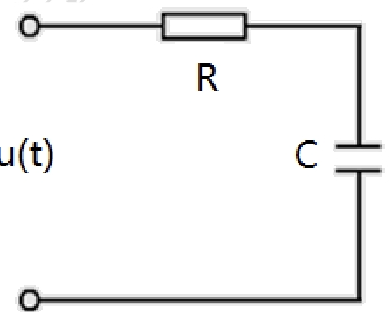
\includegraphics[width=0.4\textwidth]{RC.png}
\caption{RC串联电路}
\end{figure}

设电路中的电流为$i(t)$,根据基尔霍夫电压定律和电容的性质可以列出如下电路方程:
\begin{equation}
\begin{cases}
Ri(t)+u_c(t)=u(t)\
i(t)=C\frac{du_c(t)}{dt}
\end{cases}
\end{equation}

化简可得
\begin{equation}
\tau\frac{du_c(t)}{dt}+u_c(t)=u(t)
\end{equation}

其中$\tau\equiv RC$称为电路的时间常数。如果$u(t)$长时间保持不变,则$\frac{du_c(t)}{dt}=0$,$u_c(t)=u(t)$也保持不变。这时如果改变$u(t)$,如果改变的幅度有限,由于电容器储存的能量不能瞬时改变(功率有限),$u_c(t)$只能连续改变。假设$t<0$时$u(t)=u_0$,当$t\geq 0$时$u(t)=u_\infty$,则有
\begin{equation}
u_c(t)=
\begin{cases}
u_0 & t<0\\
u_\infty+(u_0-u_\infty)e^{-\frac{t}{\tau}} & t\geq 0
\end{cases}
\end{equation}

当$t\gg\tau$时,$u_c(t)$达到新的稳定值$u_\infty$,暂态过程完成。图2画出了一些充电($u_0=0,u_\infty=U_0$)和放电($u_0=U_0,u_\infty=0$)过程中$u_c$的变化曲线。
\begin{figure}[ht]
\centering
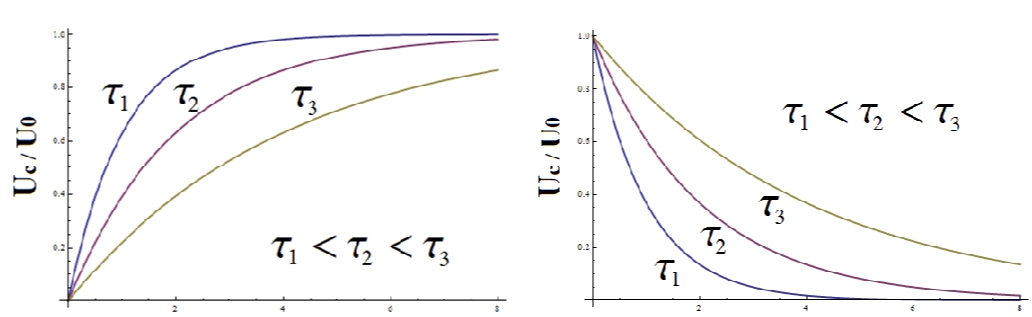
\includegraphics[width=0.8\textwidth]{RC_charge_discharge.png}
\caption{RC充电(左)和放电(右)曲线}
\end{figure}

RL串联电路(见图3)中也存在一阶暂态过程。设电路中的电流为$i(t)$,则电路方程为
\begin{equation}
Ri(t)+L\frac{di(t)}{dt}=u(t)\Rightarrow\tau\frac{di(t)}{dt}+i(t)=\frac{u(t)}{R}
\end{equation}

其中时间常数$\tau=L/R$。注意与RC电路不同,在RL电路中时间常数与$R$成反比。当总电压$u(t)$发生幅度有限的跃变时,由于电感器存储的磁场能不能发生跃变,$i(t)$将连续地变化。
\begin{figure}[htbp]
\centering
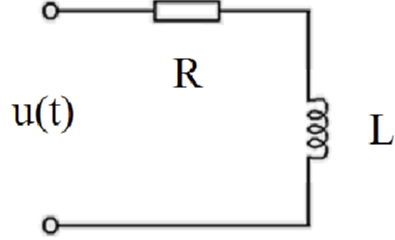
\includegraphics[width=0.4\textwidth]{RL.png}
\caption{RL串联电路}
\end{figure}

RLC串联电路(图4)在总电压突变时将产生一个典型的二阶暂态过程。
\begin{figure}[htbp]
\centering
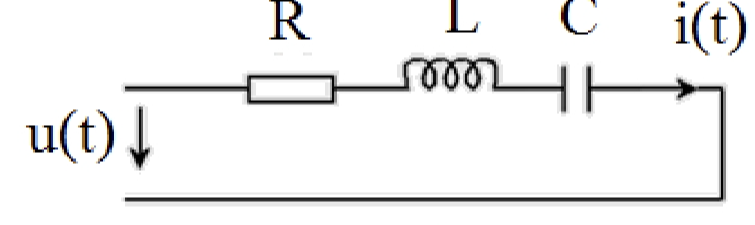
\includegraphics[width=0.4\textwidth]{RLC.png}
\caption{RLC串联电路}
\end{figure}

设电路中的电流为$i(t)$,电感、电容两端的电压分别为$u_L(t)$和$u_c(t)$,根据基尔霍夫电压定律和电感、电容的性质,可得以下电路方程:
\begin{equation}
\begin{cases}
Ri(t)+u_L(t)+u_c(t)=u(t)\
i(t)=C\frac{du_c(t)}{dt}\
u_L(t)=L\frac{di(t)}{dt}=LC\frac{d^2u_c(t)}{dt^2}
\end{cases}
\end{equation}

化简后为
\begin{equation}
LC\frac{d^2u_c(t)}{dt^2}+RC\frac{du_c(t)}{dt}+u_c(t)=u(t)
\end{equation}

这个方程可写成标准的受迫振动方程的形式:
\begin{equation}
\frac{1}{\omega_0^2}\frac{d^2u_c(t)}{dt^2}+\frac{1}{Q\omega_0}\frac{du_c(t)}{dt}+u_c(t)=u(t)
\end{equation}

其中$\omega_0=\frac{1}{\sqrt{LC}}$为固有频率,$Q=\frac{1}{R}\sqrt{\frac{L}{C}}$称为品质因数(简称Q值,Q-factor)。考虑外加电压$u(t)=0$的暂态解。令$u_c(t)=e^{j\omega t}$,带入方程得到
\begin{equation}
-\frac{\omega^2}{\omega_0^2}+j\frac{\omega}{Q\omega_0}+1=0
\end{equation}

解之得到
\begin{equation}
\omega=\omega_{1,2}=\left(j\frac{1}{2Q}\pm\sqrt{1-\frac{1}{4Q^2}}\right)\omega_0
\end{equation}

$\omega_{1,2}$(或$Q$值)决定了暂态解的衰减模式(参见图5)。
\begin{figure}[ht]
\centering
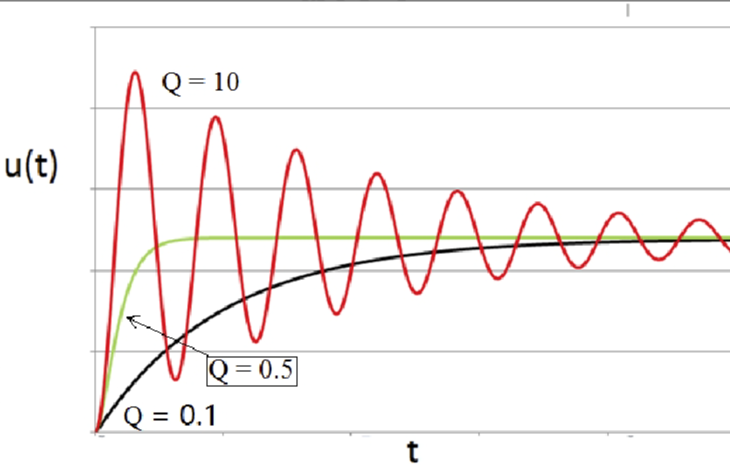
\includegraphics[width=0.8\textwidth]{RLC_damping.png}
\caption{阻尼振荡的三种形式}
\end{figure}

(1) $Q>\frac{1}{2}$,$\omega$的实部不为零,电路暂态表现为欠阻尼(under-damping),呈衰减振荡:
\begin{equation}
u_c(t)=ce^{-\text{Im}(\omega)t}\cos[\text{Re}(\omega)+\varphi]
\end{equation}

其中振荡的"角频率"
\begin{equation}
\omega'=|\text{Re}(\omega)|=\sqrt{1-\frac{1}{4Q^2}}\omega_0=\sqrt{\frac{1}{LC}-\frac{R^2}{4L^2}}
\end{equation}

振荡的"周期"$T=2\pi/\omega'$,衰减振荡的包络线为指数函数,对应时间常数
\begin{equation}
\tau=\frac{1}{\text{Im}(\omega)}=\frac{2Q}{\omega_0}=\frac{2L}{R}
\end{equation}

每振荡一周期,振幅衰减
\begin{equation}
\eta=\exp\left(-2\pi\frac{\text{Im}(\omega)}{|\text{Re}(\omega)|}\right)=\exp\left(-\frac{2\pi}{\sqrt{4Q^2-1}}\right)\approx\exp\left(-\frac{\pi}{Q}\right)
\end{equation}

上式给出实验中粗略估计$Q$值的方法:由于$e^{-\pi}=0.0432\approx 0$,如果$Q\gg 1$,大约经过$Q$次振荡后电路就达到稳态。

(2) $Q<\frac{1}{2}$,$\omega$为纯虚数,电路暂态表现为过阻尼(over-damping),呈双指数衰减:
\begin{equation}
u_c(t)=c_1e^{-\frac{t}{\tau_1}}+c_2e^{-\frac{t}{\tau_2}}
\end{equation}

其中
\begin{equation}
\tau_{1,2}=\frac{1}{\text{Im}(\omega_{1,2})}=\frac{2Q}{\omega_0(1\pm\sqrt{1-4Q^2})}=\frac{1}{2(1\mp\sqrt{1-4Q^2})}RC
\end{equation}

衰减的特征时间主要由较长的那个时间常数决定,即$\tau=\max{\tau_1,\tau_2}$。注意$\tau_1+\tau_2=RC$。

(3) $Q=\frac{1}{2}$,临界阻尼(critical-damping),$\omega_1=\omega_2=j\omega_0$,$u_c(t)$的衰减形式为
\begin{equation}
u_c(t)=(c_1+c_2t)e^{-\frac{t}{\tau}}
\end{equation}

其中$\tau=1/\omega_0$。

容易证明,如果固定$L,C$而改变$R$(即保持$\omega_0$不变而改变$Q$),在$Q=1/2$,即$R=2\sqrt{\frac{L}{C}}\equiv R_c$时,$\tau$取到最小值$\tau_{\min}=1/\omega_0$。



\section{实验过程}

\subsection{测量RC放电曲线,计算时间常数}

\begin{enumerate}
\item 搭建如图6所示的RC电路,选取合适的$R$、$C$值,使时间常数$\tau=RC$在毫秒量级。
\item 示波器CH1观察信号发生器输出(方波),CH2观察电容两端电压。分别调节信号发生器和示波器的参数,使波形稳定可观察。
\item 调节示波器时基,使波形充满屏幕。调节垂直位移,使波形上下对称。
\item 用光标测量功能,测量并记录一个周期内的若干个点${t_i,u_i}$(或直接导出波形数据)。
\item 选取其中的放电段数据,用指数衰减模型$u_i=Ae^{-Bt_i}$拟合,得到最佳参数$B$,则时间常数$\tau=1/B$。
\end{enumerate}

\begin{figure}[htbp]
\centering
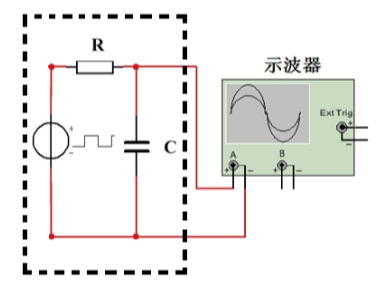
\includegraphics[width=0.4\textwidth]{RC_test.png}
\caption{RC放电测试电路}
\end{figure}

\subsection{测量RL放电曲线,计算时间常数(选做)}

步骤与RC放电实验类似,只需将电容换成电感即可。注意选取合适的$R$、$L$值,使时间常数$\tau=L/R$在毫秒量级。

\subsection{测量RLC欠阻尼振荡,计算固有频率和品质因数}

\begin{enumerate}
\item 搭建如图6所示的RLC串联电路,并选取合适的$R$、$L$、$C$值,使得$Q=\frac{1}{R}\sqrt{\frac{L}{C}}>\frac{1}{2}$,即欠阻尼情况。
\item 用示波器观察电容两端电压波形,调节示波器时基使波形稳定且几个周期充满屏幕。
\item 用光标测量相邻两个波峰之间的时间间隔$\Delta t$,则周期$T=\Delta t$,固有频率$f_0=\frac{1}{T}$。
\item 测量第$k$个波峰与波谷的电压差$\Delta_k$,则相邻两个峰谷电压差之比为衰减系数
\begin{equation}
\eta=\frac{\Delta_{k+1}}{\Delta_k}=\exp\left(-\frac{2\pi}{\sqrt{4Q^2-1}}\right)\approx\exp\left(-\frac{\pi}{Q}\right)
\end{equation}
\item 由此可估算品质因数$Q\approx\frac{\pi}{\ln(1/\eta)}$。
\end{enumerate}

\begin{figure}[htbp]
\centering
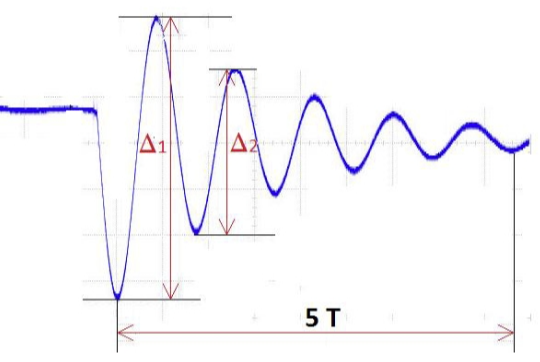
\includegraphics[width=0.4\textwidth]{RLC_oscillation}
\caption{欠阻尼振荡波形测量}
\end{figure}

\subsection{观察RLC不同阻尼模式,测量临界电阻}

\begin{enumerate}
\item 固定$L$、$C$,改变$R$(比如用电位器),观察并记录波形从欠阻尼到过阻尼的变化过程。
\item 仔细调节$R$,使波形处于临界阻尼状态,读出此时的$R_c$值。
\item 比较实测的临界电阻$R_c$与理论值$2\sqrt{L/C}$,分析误差来源。
\end{enumerate}

\begin{figure}[htbp]
\centering
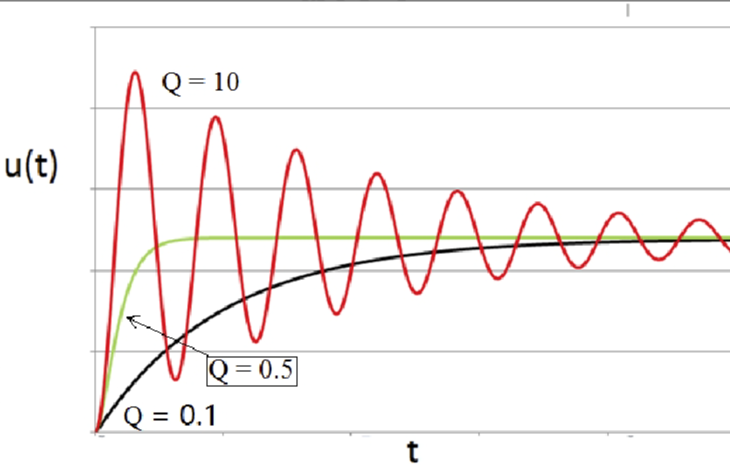
\includegraphics[width=0.4\textwidth]{RLC_damping.png}
\caption{RLC串联电路的三种阻尼模式}
\end{figure}
\newpage
\section{预习思考题}

\begin{enumerate}
\item 电容储存电场能量,电感储存磁场能量。设电容两端电压为$U$,电容值为$C$,则储存的电场能量为
\begin{equation}
W_e=\frac{1}{2}CU^2
\end{equation}

设电感两端电流为$I$,电感值为$L$,则储存的磁场能量为
\begin{equation}
W_m=\frac{1}{2}LI^2
\end{equation}

\item 在RLC串联电路的二阶暂态过程中,固有频率为$\omega_0=\frac{1}{\sqrt{LC}}$,品质因数为$Q=\frac{1}{R}\sqrt{\frac{L}{C}}$。如果保持$L$、$C$不变而改变$R$,则$\omega_0$不变而$Q$变化。根据前面的推导,欠阻尼情况下的特征衰减时间为
\begin{equation}
\tau=\frac{1}{\text{Im}(\omega)}=\frac{2Q}{\omega_0}=\frac{2RC}{\sqrt{1-4Q^2}}
\end{equation}

令$\frac{d\tau}{dQ}=0$,解得
\begin{equation}
Q=\frac{1}{2}
\end{equation}

此时$\tau$取得最小值
\begin{equation}
\tau_{\min}=\frac{1}{\omega_0}=\sqrt{LC}
\end{equation}

\item RLC串联电路的微分方程为
\begin{equation}
LC\frac{d^2u_c(t)}{dt^2}+RC\frac{du_c(t)}{dt}+u_c(t)=u(t)
\end{equation}

阻尼弹簧振子的动力学方程为
\begin{equation}
m\frac{d^2x(t)}{dt^2}+b\frac{dx(t)}{dt}+kx(t)=F(t)
\end{equation}

其中$m$为质量,$b$为阻尼系数,$k$为弹簧劲度系数,$F(t)$为外力。

比较两个方程可知,对应关系为:
\begin{itemize}
\item 电容$C$对应于$1/k$,即弹簧劲度系数的倒数
\item 电感$L$对应于质量$m$
\item 电阻$R$对应于阻尼系数$b$
\item 电容两端电压$u_c(t)$对应于位移$x(t)$
\item 外加电压$u(t)$对应于外力$F(t)$
\end{itemize}

从物理意义上看,这种对应关系也是合理的:
\begin{itemize}
\item 电容对应于弹性势能的储存,类似于弹簧
\item 电感对应于磁场能量(动能)的储存,类似于质量
\item 电阻对应于电能的耗散,类似于阻尼
\end{itemize}
\end{enumerate}

\end{document}
